%Correctness
\section{Correctness}
\subsection{The Graph Structure}
\begin{figure}[htb]
    \centering
    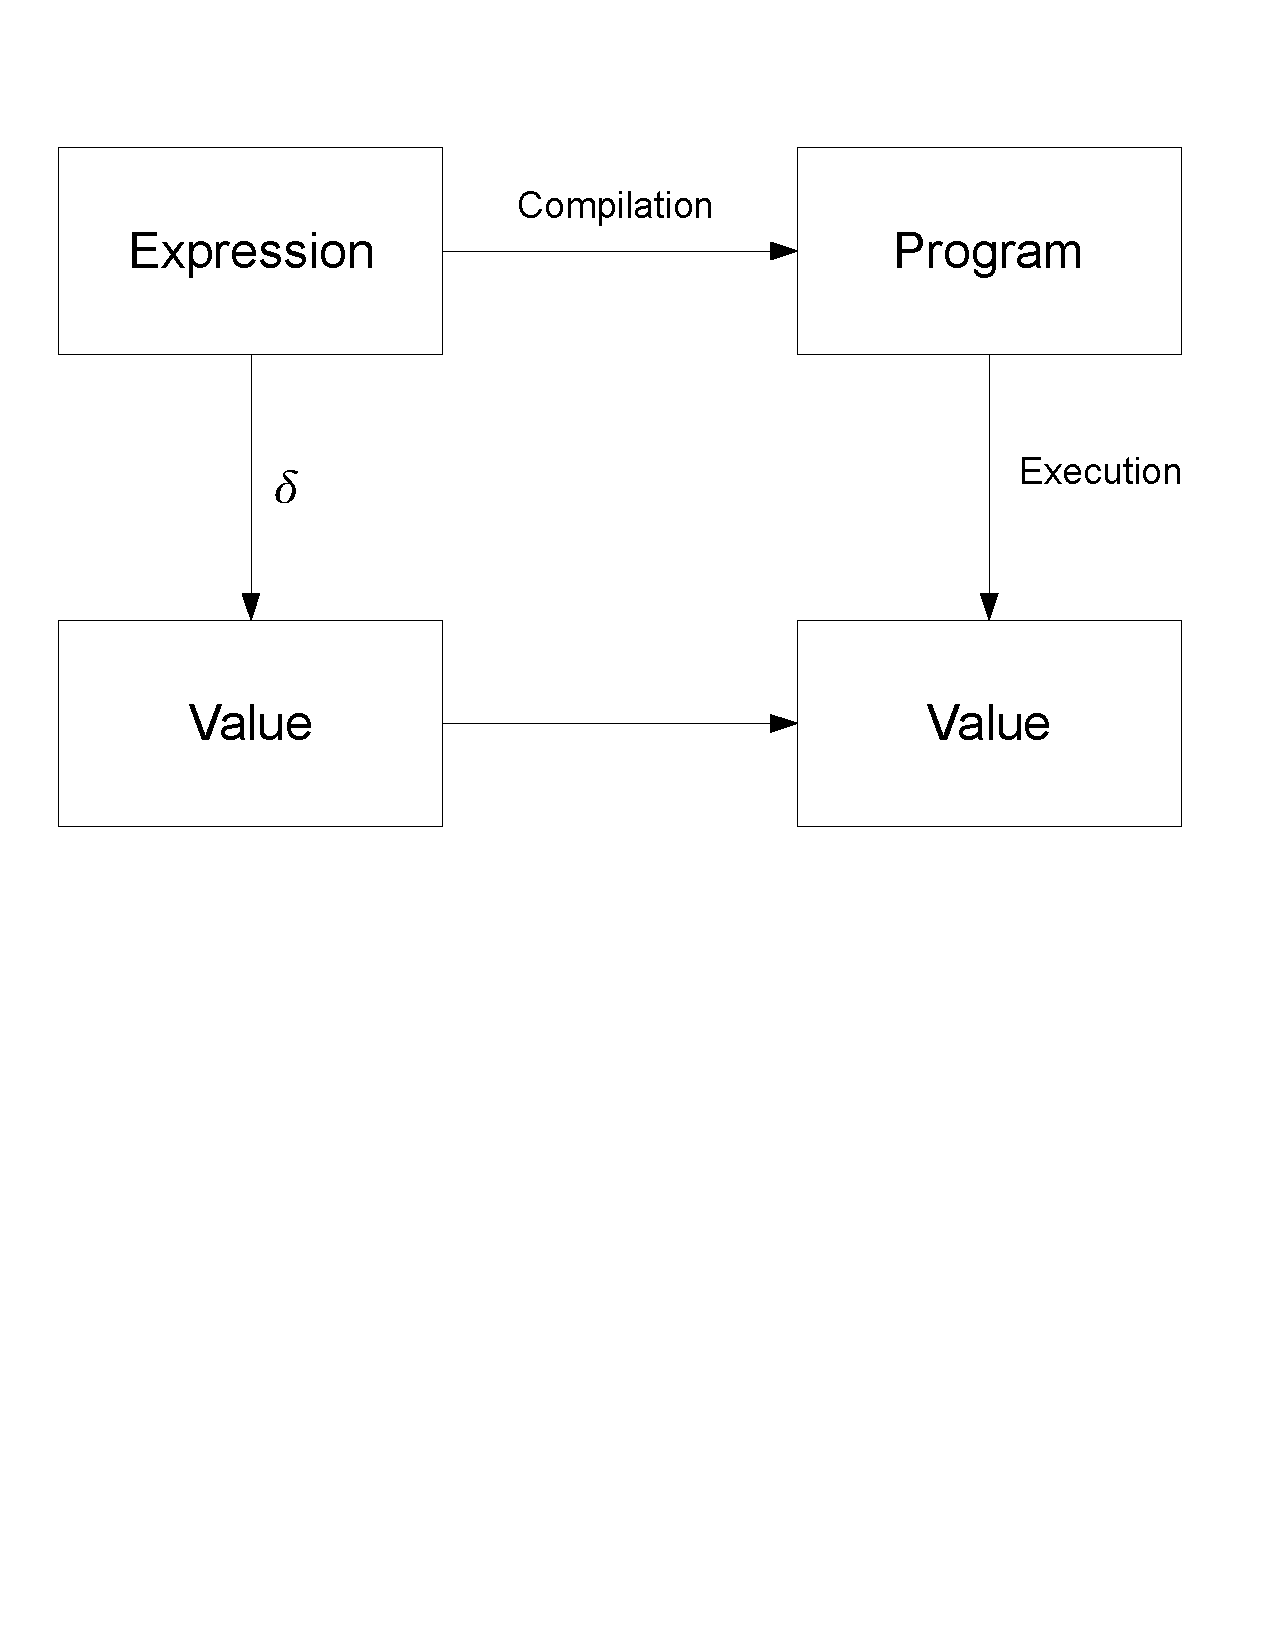
\includegraphics[trim= 10mm 120mm 10mm 10mm, clip, width=250px]{./images/correctness_graph1.pdf}
    \caption{Code Transformations}
    \label{fig:correctness_graph1}
\end{figure}
The graph structure chosen is simple directed graph in which the syntax and semantics are discussed in detail in sections \ref{sec:statechartsyn}, \ref{sec:statechartsem} respectively. Our program preforms transformations on the diagram to form code constructs. In order to show correctness we will demonstrate that our transformations follow figure \ref{fig:correctness_graph1}. Figure \ref{fig:correctness_graph1} essentially says that a simulated evaluation of each expression ($\delta$) to a value will be equivalent to the actual executed program of the same value. In addition we also need to prove the program structure
\begin{figure}[htb]
    \centering
    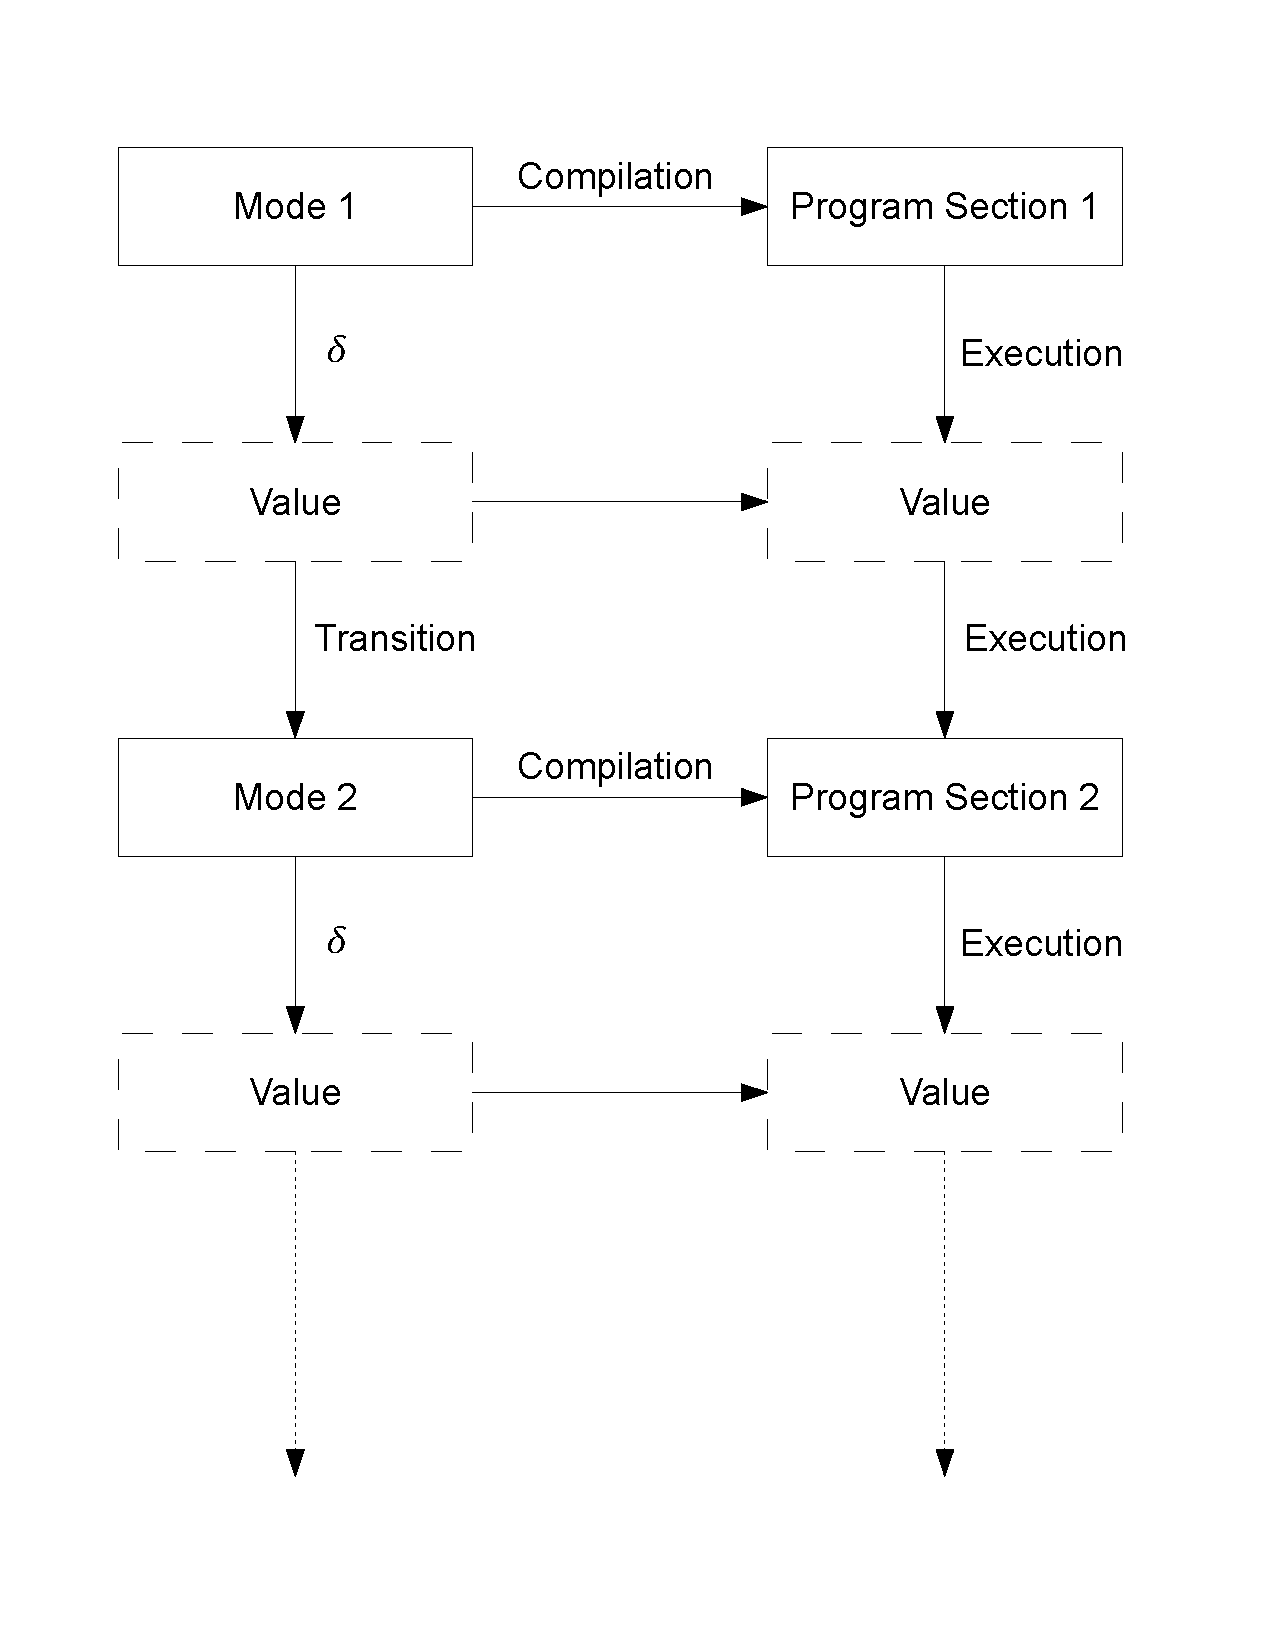
\includegraphics[trim= 10mm 30mm 10mm 10mm, clip, width=\imgmedium]{./images/correctness_graph2.pdf}
    \caption{Code Transition Structure}
    \label{fig:correctness_graph2}
\end{figure}
generated from an graph structure is correct. To do so we extend figure \ref{fig:correctness_graph1} iteratively to obtain figure \ref{fig:correctness_graph2} to evaluate the transitions.

In this section we will begin by showing that each of the transformations are correct by constructing basic atoms. We will start by looking at atoms that have the simplest expressions first. The simplest of these is a diagram in which only the start node exists as shown in \ref{fig:correctness_ex_start}.

\begin{figure}[htb]
	\centering
	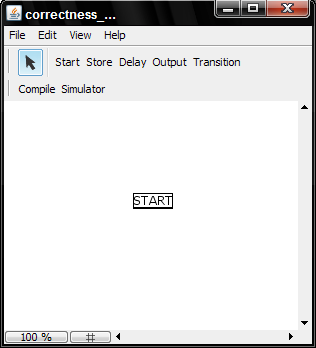
\includegraphics[width=\imgmedphoto]{./images/correctness_ex_start.png}
	\caption{Singular Start Block}
	\label{fig:correctness_ex_start}
\end{figure}
In this simple example the following generated intermediate code \emphasize{IL} is created.

\begin{minipage}{\textwidth}
\begin{lstlisting}[frame=single]
// VARIABLE DECLARATIONS //
BLUID0:
//////////////////////////////////////
//        PROGRAM START             //
//////////////////////////////////////
goto EOF;

EOF:
return;
\end{lstlisting}
\end{minipage}

In this simplest example we have a label inserted at the beginning of the start block so we can re-enter the start block namely BLUID0. Following the label a comment header to denote the block type, and no variables declared.  Because there is no other transition or block an automatic transition to \emphasize{EOF} is setup in order to terminate the program. In our system this is analogous to "staying in a state indefinitely" as the behaviour after return is executed is to just halt the chip.

\begin{figure}[htb]
	\centering
	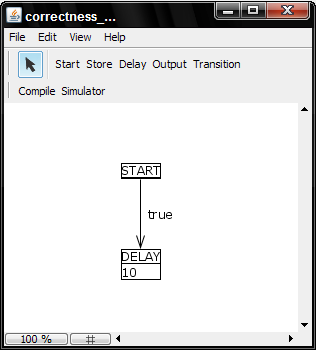
\includegraphics[width=\imgmedphoto]{./images/correctness_ex_delay.png}
	\caption{Delay Block}
	\label{fig:correctness_ex_delay}
\end{figure}

Moving up in complexity we have a start block followed by our next simplest element the delay block, joined by one transition leaving the start block. We can see from figure \ref{fig:correctness_ex_delay}
the structure of this new graph. We will use this example to examine transitions are compiled into final code, but first we shall look at the delay block itself.

\begin{minipage}{\textwidth}
\begin{lstlisting}[frame=single]
// VARIABLE DECLARATIONS //
...

BLUID1:
//////////////////////////////////////
//        DELAY                     //
//////////////////////////////////////
delayms(10);
goto EOF;

EOF:
return;
\end{lstlisting}
\end{minipage}

The delay block itself has a structure identical to the start block. The only difference in this case is the delay block doesn't have a null code section. The delay block generates one line of code, namely delay(integer). The actual delay routine is implemented on the driver level per device since certain devices lack internal timers. It will be up to each implementer to ensure that the delay will correctly delay each the integer specified (in milliseconds). 

\begin{minipage}{\textwidth}
\begin{lstlisting}[frame=single]
// VARIABLE DECLARATIONS //
BLUID0:
//////////////////////////////////////
//        PROGRAM START             //
//////////////////////////////////////
goto BLUID1;
goto EOF;

BLUID1:
//////////////////////////////////////
//        DELAY                     //
//////////////////////////////////////
delayms(10);
goto EOF;

EOF:
return;
\end{lstlisting}
\end{minipage}

In the example shown in figure \ref{fig:correctness_ex_delay} a transition can be seen. The reader will observe that we have directly mapped each edge to a goto statement that is guarded by the guard condition on the edge itself. As defined in section \ref{sec:statechartsyn} the transitions are always mutually exclusive and to not do so would be considered a syntax error. The reason is there is no way to enforce sequence in which each edge is evaluated that would make sense to the programmer constructing the diagram in a visual way. It is up to the programmer (diagram constructor) to ensure that we never run into a condition where two edges actually have an area of overlap. This is not a problem for our simple case as shown in figure \ref{fig:correctness_ex_delay} as we only have one edge leaving the delay block.

Each block has an unique identifier associated with it, this identifier is what is used by the goto blocks in order to recreate the graph structure in the code. The unique identifier is generated at design time and is checked at compile time to ensure that it is in fact unique.

Next we look at the output block. The new item introduced by the output block are variables. The output block during its run will need to set a value to a variable. It does this in order to update the output on the port. 

\begin{figure}[htb]
	\centering
	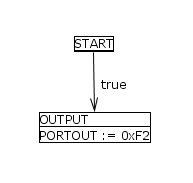
\includegraphics[width=\imgmedphoto]{./images/correctness_ex_output.png}
	\caption{Output Block}
	\label{fig:correctness_ex_output}
\end{figure}

The resulting compiled output from figure \ref{fig:correctness_ex_output} is shown below.

\begin{minipage}{\textwidth}
\begin{lstlisting}[frame=single]
// VARIABLE DECLARATIONS //
BLUID2:
//////////////////////////////////////
//        PROGRAM START             //
//////////////////////////////////////
goto BLUID3;
goto EOF;

BLUID3:
//////////////////////////////////////
//        OUTPUT                    //
//////////////////////////////////////
PORTOUT = 0xF2;
goto EOF;

EOF:
return;
\end{lstlisting}
\end{minipage}

The reader will note that we did not change any of the transitions from figure \ref{fig:correctness_ex_delay}. Despite this the BLUID's are still different. It is easy to see that the "goto" routing structure still behaves the same way despite having different labels. We note that the output block's "set" operation as shown in figure \ref{fig:correctness_ex_output} becomes translated to "PORTOUT = 0xF2;" in the final intermediate language code. The right hand side of the equation can be any valid expression and is not just limited to an costant as shown here. Since the right hand side is transfered verbatim into the final code what the diagram creator draws essentially becomes exactly what is written in the final code.

In order to examine transitions in more detail we need to look at logic on transitions. So far because all transitions have been guarded with he condition "true" or always taken we have not had the opportunity to see any guard conditions in the code. Instead in the our current code we only observe a always taken goto statement at the end. We will construct a basic diagram with our next component the "Store Block" to demonstrate how guard conditions are enumerated as well as demonstrate another basic primitive block that allows the diagram creator to set internal variables and perform calculations.

\begin{figure}[htb]
	\centering
	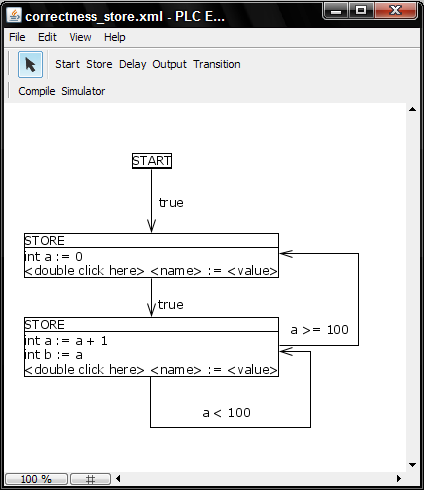
\includegraphics[width=\imgmedphoto]{./images/correctness_ex_store.png}
	\caption{Store Block Example}
	\label{fig:correctness_ex_store}
\end{figure}

The resulting code from figure \ref{fig:correctness_ex_store} is shown below:

\begin{minipage}{\textwidth}
\begin{lstlisting}[frame=single]
// VARIABLE DECLARATIONS //
int a;
int b;
BLUID0:
//////////////////////////////////////
//        PROGRAM START             //
//////////////////////////////////////
goto BLUID1;
goto EOF;

BLUID1:
//////////////////////////////////////
//        STORE                     //
//////////////////////////////////////
a = 0;

goto BLUID2;
goto EOF;

BLUID2:
//////////////////////////////////////
//        STORE                     //
//////////////////////////////////////
a = a + 1;
b = a;

if (a >= 100) goto BLUID1;
if (a < 100) goto BLUID2;
goto EOF;

EOF:
return;
\end{lstlisting}
\end{minipage}

First we look at the first store block with "BLUID1" as its label. We can easily see that from our diagram of transformations in figure \ref{fig:correctness_graph1} that our expression "$a := 0$" through the compile transformation was converted to "$a = 0$". Taking the transformation in figure \ref{fig:correctness_graph1} of "$\delta$" we note that the meaning of "$a := 0$" is that the value of $\delta(a) = 0$. Similarily executing "$a = 0$" in C we find that after execution the value of $exec(a) = 0$. Since the mapping from our semantic "value" to our executed "value" is the same we can conclude that the mapping is correct as by our definition. Next we the second store block with "BLUID2" as its label. From the diagram in figure \ref{fig:correctness_ex_store} the second store block has two notable differences. The first is that it has more than one set operation, and the second is that it uses variables in its expression and not just constants. As stated before the right hand side allows for any expression to be placed. From our definitions in section \ref{sec:statechartsem} of \plcchart it is understood that each expression forumlae is understood to occur in sequence. In this example "$a := a + 1$" will occur before "$b := a$". To demonstrate correctness we once again refer to figure \ref{fig:correctness_graph1} and start with our first expression. We note that after compilation $a := a + 1$ is compiled to $a = a + 1$, and $b := a$ becomes $b = a$. We can see that $\delta(a) = a + 1, \delta(b) = a + 1$, similarly $exec(a) = a + 1, exec(b) = a + 1$. Since mapping from $\delta(a) \rightarrow exec(a)$ and $\delta(b) \rightarrow exec(b)$ we can conclude that the transformation preserves the meaning of the values and thus is correct to the semantics outlined in sectin \ref{sec:statechartsem}.

To show the correctness of guarded transitions we now look at figure \ref{fig:correctness_graph2}. Note that figure \ref{fig:correctness_graph2} shares most of it's structure with figure \ref{fig:correctness_graph1} but is annotated to include transitions and modes. A mode as established in section \ref{sec:statechartsem} is similar to a state or a block in our diagram. Our diagrams always begin from the "start" node, similarily our begins its execution from "BLUID0" in the above code which is the compiled code. No values are updated in our start block so we can take the transition leaving the start node this puts us into the first store block (which we will refer to as $Store_1$ for disambiguity). On the execution side we see that at the end of the start code block we have the line \texttt{goto BLUID1;} we can note that BLUID1 points to the code block for our store in the diagram. We can conclude that $Transition(Start, true) \rightarrow Store_1$ similarily $Execution(Start, true) \rightarrow Store_1$. Thus we can conclude that transitions leaving "start" are correct. A similar argument can be made for $Store_1$ since no transitions are guarded.

For the guarded transitions in our second store block which we will refer to as $Store_2$ with "BLUID2" we must look at each guarded condition. We have previously proven for figure \ref{fig:correctness_ex_store} that figure \ref{fig:correctness_graph1} holds so we will skip that proof here. Extracting all edges leaving $Store_2$ we obtain $Transition(Store_2, a >= 100) \rightarrow Store_1$ and $Transition(Store_2, a < 100) \rightarrow Store_2$. Now all that remains is to show that the execution code has the same transitions. We can see from the compiled code that at the end of our $Store_2$ code block we have a series of "if" statements. We can see that \texttt{if (a >= 100) goto BLUID1;} is equivalent to $Transition(Store_2, a >= 100) \rightarrow Store_1$ and \texttt{if (a < 100) goto BLUID2;} is equivalent to $Transition(Store_2, a < 100) \rightarrow Store_2$. In this way we have demonstrated that guarded conditions are correct as well.


By demonstrating that our system is correct both in compilation and execution with respect to figures \ref{fig:correctness_graph1} and \ref{fig:correctness_graph2}. We can conclude that our system is functionally correct by its construction and design.

%the lower sections might be superceeded by the above.
%\subsection{The IL}
%\subsection{The Generated Code Sections}
%\subsection{The Simulator}